\documentclass[runningheads]{llncs}
%
\usepackage[T1]{fontenc}
\usepackage[utf8]{inputenc}
% Se escrever em português, descomente a linha seguinte:
%\usepackage[portuguese]{babel}
\usepackage{newtxtext}
\usepackage[varvw]{newtxmath}
\usepackage{graphicx}
\usepackage{amsmath}
\usepackage{array}
\usepackage{cite}
\usepackage{tikz}
\usetikzlibrary{arrows.meta}
% \usepackage{color}
% \renewcommand\UrlFont{\color{blue}\rmfamily}
% \urlstyle{rm}

\begin{document}

\title{A Decision Support System for Prioritising Industrial Maintenance Interventions}
\titlerunning{DSS for Prioritising Industrial Maintenance Interventions}

\author{Artur Alves\inst{1} (1250496) \and
Lucas Fernandes\inst{1} (1252052) \and
Ricardo Pereira\inst{1} (1250548)}
%
\authorrunning{A. Alves et al.}
%
\institute{Instituto Superior de Engenharia do Porto (ISEP),\\
Rua Dr. António Bernardino de Almeida, 431, 4249-015 Porto, Portugal \\
\email{\{1250496,1252052,1250548\}@isep.ipp.pt}}

\maketitle

\begin{abstract}
% 150--250 palavras
Industrial plants often have more pending maintenance interventions than technicians, spare parts and downtime windows can absorb, so their order has to be decided. Following the Kitchenham guidelines and the PRISMA 2020 statement, 554 records from IEEE Xplore and Web of Science (2021--2026) were screened and 31 studies with evaluation in a real setting were analysed for their criteria, methods, system architecture and validation. Resource constraints, failure likelihood and production impact dominate the criteria, while safety is explicit in only seven studies and is usually traded off against cost. Few proposals are implemented systems, priorities are rarely updated or explained, and only six were tested in the plant. Based on these gaps, we propose a decision support system that combines machine learning failure prediction with AHP and TOPSIS, treats safety as a non-compensable constraint and explains each position in the ranking.

\keywords{Industrial maintenance \and Decision support systems \and Maintenance prioritisation \and Multi-criteria decision-making \and Predictive maintenance.}
\end{abstract}

\section{Introdução}
Enquadramento, motivação, objetivos da revisão e estrutura do artigo.

\section{Metodologia da Revisão}
\subsection{Questões de investigação}
\subsection{Bases de dados e strings de pesquisa}
\subsection{Critérios de inclusão e exclusão}
\subsection{Processo de seleção (PRISMA)}

\section{Background: Maintenance Strategies}
\label{sec:background}

Maintenance strategies differ in what triggers an intervention and in the information they require (Table~\ref{tab:strategies}, Appendix~\ref{app:figures}). \textbf{Corrective} maintenance restores equipment after a failure; it needs no planning but exposes the plant to unplanned downtime and safety risks. \textbf{Preventive} maintenance acts at fixed time or usage intervals, which is easy to plan but ignores the state of each machine, so some components are replaced too early and others fail first. \textbf{Condition-based} maintenance (CBM) intervenes when a measured indicator, such as vibration or temperature, crosses a threshold. \textbf{Predictive} maintenance goes further and estimates the remaining useful life (RUL) with data-driven, physics-based or hybrid models. A RUL estimate, however, does not say which of several pending interventions should come first, nor how to weigh failure likelihood against safety, production or cost; many retrieved studies stopped at this stage and were excluded under E4. \textbf{Prescriptive} maintenance closes this gap by recommending the action, its timing and its resources, combining predictions with costs, constraints and expert knowledge. This is the level at which the present work is placed.

Two management frameworks are often combined with these strategies. Reli\-a\-bil\-i\-ty-Centred Maintenance (RCM) defines the policy of each asset through an analysis of its functions, failure modes and consequences; its tools, FMEA and criticality analysis, introduced the ranking of assets by severity and likelihood that underlies many of the models in Section~\ref{sec:criteria-methods}. Total Productive Maintenance (TPM) involves operators in equipment care and measures performance through Overall Equipment Effectiveness (OEE), bringing the production cost of downtime into maintenance decisions.
\section{Critérios e Métodos de Priorização}
\label{sec:criterios}

\subsection{Critérios de priorização}
Apresentar os critérios mais usados na literatura, idealmente numa pequena tabela com as referências que usam cada um.
Os critérios mais recorrentes incluem a criticidade do equipamento, o impacto na segurança, o impacto na produção, o custo da intervenção, a probabilidade de falha, o histórico de falhas, a redundância e a disponibilidade de recursos. Rastogi et al.~\cite{rastogi2024} identificam nove fatores de avaliação, embora apenas quatro sejam efetivamente usados no seu modelo.

\subsection{Análise de criticidade e FMEA}
Matrizes de criticidade, FMEA e o Risk Priority Number (RPN = severidade $\times$ ocorrência $\times$ deteção); limitações conhecidas do RPN.

\subsection{Métodos de decisão multicritério}
Para cada método, uma ou duas frases sobre como funciona e um exemplo de aplicação à manutenção:
\begin{itemize}
  \item \textbf{Definição de pesos:} AHP, BWM.
  \item \textbf{Ordenação de alternativas:} soma ponderada, TOPSIS, VIKOR, PROMETHEE, ELECTRE.
  \item \textbf{Variantes fuzzy:} tratamento da incerteza nos julgamentos dos especialistas.
\end{itemize}

\subsection{Otimização e escalonamento}
Programação matemática, meta-heurísticas (ex.: PSO, algoritmos genéticos) e escalonamento com restrições de recursos e janelas de paragem.
\section{Sistemas de Apoio à Decisão em Manutenção}
\subsection{Arquiteturas e componentes}
\subsection{Integração de dados (CMMS, ERP, SCADA, IoT)}
\subsection{Casos de aplicação industrial}

\section{Análise Crítica, Lacunas e Tendências}
\label{sec:analise}
 
\subsection{Comparação das abordagens}
 
A Tabela~\ref{tab:comparacao} resume os trabalhos analisados. As abordagens dividem-se em dois grupos. O primeiro combina a previsão do estado dos equipamentos com uma ordenação multicritério estática, como o modelo de Rastogi et al.~\cite{rastogi2024}. Estas abordagens são transparentes e fáceis de aplicar, mas dependem de pesos definidos pelos autores e produzem uma ordenação válida apenas para o momento em que é calculada. O segundo grupo trata a priorização como um problema sequencial, como o modelo de aprendizagem por reforço de Luo~\cite{luo2026}. Estas abordagens consideram o efeito das decisões atuais no estado futuro do sistema, mas funcionam como uma caixa preta e exigem um ambiente de simulação difícil de construir e validar.
 
\begin{table}[htbp]
\centering
\caption{Comparação dos trabalhos analisados.}
\label{tab:comparacao}
\begin{tabular}{|p{1.1cm}|p{3.0cm}|p{2.3cm}|p{4.0cm}|}
\hline
\textbf{Ref.} & \textbf{Método} & \textbf{Dados e validação} & \textbf{Limitações} \\
\hline
\cite{rastogi2024} & Previsão da RUL e soma ponderada de fatores, com restrições de recursos & Caso ilustrativo de um sistema elétrico & Pesos hipotéticos; sem método multicritério formal; segurança fora do modelo \\
\hline
\cite{luo2026} & Aprendizagem por reforço (Deep Q-Network) & Dataset público e caso de um parque eólico & Ambiente pouco descrito; comparações discutíveis; sem explicação das decisões \\
\hline
\end{tabular}
\end{table}
 
\subsection{Lacunas identificadas}
 
Da análise realizada resultam as seguintes lacunas:
\begin{itemize}
  \item \textbf{Pesos pouco justificados.} Os pesos dos critérios são muitas vezes definidos pelos autores, sem recurso a métodos estruturados de elicitação junto dos especialistas~\cite{rastogi2024}.
  \item \textbf{Segurança tratada como compensável.} A segurança surge como mais um peso, o que permite que um ganho em custo ou disponibilidade compense um risco para as pessoas~\cite{rastogi2024,luo2026}.
  \item \textbf{Validação limitada.} Os resultados assentam em dados ilustrativos ou pouco documentados, sem comparação com as práticas usadas na indústria.
  \item \textbf{Falta de explicação.} O decisor recebe uma pontuação ou uma ação recomendada, mas não percebe porque é que uma intervenção ficou à frente de outra~\cite{luo2026}.
  \item \textbf{Decisão individual.} As abordagens assumem um único decisor, embora a priorização envolva normalmente as áreas de manutenção, produção e segurança.
\end{itemize}
 
\subsection{Tendências}
 
A literatura aponta para a integração destes sistemas com gémeos digitais, que permitem testar decisões num modelo virtual do equipamento antes de as aplicar. Destaca-se também o uso de técnicas de inteligência artificial explicável, que tornam as recomendações compreensíveis para o decisor, e a passagem da manutenção preditiva para a prescritiva, em que o sistema não se limita a prever a falha e recomenda a ação a tomar. Por fim, os sistemas multiagente e de decisão em grupo surgem como forma de conciliar os interesses das várias áreas envolvidas.

\section{Proposal}
\label{sec:proposta}

We propose a decision support system that helps the maintenance manager decide the order in which pending interventions should be carried out. The system combines the predicted failure probability of each asset with a multi-criteria decision method and returns a justified ranking. Its design follows the gaps identified in Section~\ref{sec:analysis}: safety is a non-compensable constraint (G1), criteria weights are elicited from several stakeholders through a structured method and can be tested for sensitivity (G4), and every position in the ranking is explained in terms of the criteria (G5). The ranking is recomputed when new condition data or failures arrive, which partly addresses G3, and the history of decisions is stored so that their outcomes can later be assessed (G6). Joint ranking and scheduling of interventions (G2) is left for future work.

\subsection{System Context}
\label{sec:context}

\begin{itemize}
  \item \textbf{Target users.} The main user is the maintenance manager or planner. Production and safety managers take part in defining the importance of the criteria.
  \item \textbf{Type of problem.} Semi-structured: part of the information is quantitative (condition data, costs, repair times) and part depends on expert judgement.
  \item \textbf{Synchronous and asynchronous decision.} The ranking is produced asynchronously, at the start of each shift, and recomputed whenever an urgent failure is reported. The definition of weights is a synchronous group activity, repeated when priorities in the plant change.
  \item \textbf{Criteria.} Safety risk is mandatory and cannot be relaxed: interventions with a risk to people are always placed first. Failure probability, production impact, cost, intervention duration and availability of technicians and spare parts can be relaxed and compensate each other.
  \item \textbf{Social aspects.} Maintenance, production and safety staff have different priorities. Each states its own judgements, and the system aggregates them and shows where they diverge.
  \item \textbf{Sensors.} Condition data such as temperature, vibration and torque feed the failure prediction. The prototype will use a public predictive maintenance dataset; validation with real plant data is planned as future work.
  \item \textbf{Interface.} A web application showing the ranking, the explanation of each position and a what-if view where the user changes the weights and sees the effect on the ranking.
  \item \textbf{Technologies.} Machine learning to estimate failure probability, AHP to derive the weights, and TOPSIS to rank the interventions.
\end{itemize}

\subsection{Requirements}
\label{sec:requirements}

Table~\ref{tab:requirements} lists the functional (FR) and non-functional (NFR) requirements and, where applicable, the gap from Section~\ref{sec:gaps} that each one addresses.

\begin{table}[!b]
\centering
\caption{Functional and non-functional requirements of the proposed system.}
\label{tab:requirements}
\scriptsize
\begin{tabular}{|p{0.9cm}|>{\raggedright\arraybackslash}p{9.0cm}|c|}
\hline
\textbf{ID} & \textbf{Requirement} & \textbf{Gap} \\
\hline
FR01 & Import pending interventions, equipment data and work orders (e.g., from CSV files or a CMMS). & -- \\
FR02 & Estimate the failure probability of each asset from its condition data. & -- \\
FR03 & Let each stakeholder define the importance of the criteria through pairwise comparisons, warn when judgements are inconsistent (\textit{CR} $\geq 0.1$) and aggregate the judgements of all stakeholders. & G4, G5 \\
FR04 & Place every intervention with a safety risk at the top of the list, regardless of the other criteria. & G1 \\
FR05 & Rank the remaining pending interventions and recompute the ranking when new data or failures arrive. & G3 \\
FR06 & Explain each position by showing the contribution of each criterion. & G5 \\
FR07 & Show how the ranking changes when the weights are changed (sensitivity analysis). & G4 \\
FR08 & Store each ranking, the decision taken and, later, its outcome. & G6 \\
\hline
NFR01 & Performance: produce the ranking in a few seconds for a few hundred interventions. & -- \\
NFR02 & Usability: be understandable by users without knowledge of MCDM methods. & -- \\
NFR03 & Transparency: no recommendation is shown without its justification. & G5 \\
NFR04 & Interoperability: import data in common formats and allow connection to a CMMS. & -- \\
NFR05 & Security: require authentication, with separate profiles for managers and other users. & -- \\
\hline
\end{tabular}
\end{table}

\subsection{Conceptual Architecture}
\label{sec:architecture}

The architecture (Fig.~\ref{fig:arquitetura}) has five modules. The \textbf{data module} collects condition data, work orders, costs and stock levels. The \textbf{predictive module} estimates the failure probability of each asset with a machine learning model. The \textbf{weighting module} collects the pairwise comparisons of each stakeholder, checks their consistency and aggregates them into a single set of AHP weights. The \textbf{decision module} first separates the interventions that involve a safety risk and then ranks all interventions with TOPSIS, keeping the safety-critical ones at the top. The \textbf{interface} presents the ranking, the explanation of each position and the sensitivity analysis, and records the decision taken, which feeds back into the data module.

\begin{figure}[t]
\centering
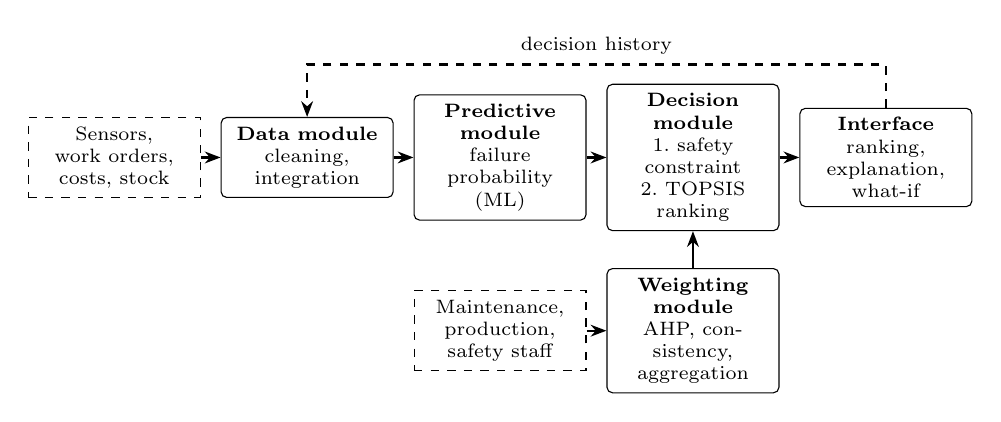
\begin{tikzpicture}[
  font=\scriptsize,
  box/.style={draw, rounded corners=2pt, align=center, minimum height=0.95cm, text width=1.95cm},
  src/.style={draw, dashed, align=center, minimum height=0.6cm, text width=1.95cm},
  arr/.style={-{Stealth[length=2mm]}, thick}
]
\node[src] (sources) at (0,0) {Sensors, work orders, costs, stock};
\node[box] (data)  at (2.45,0) {\textbf{Data module}\\ cleaning,\\ integration};
\node[box] (pred)  at (4.9,0) {\textbf{Predictive module}\\ failure\\ probability (ML)};
\node[box] (dec)   at (7.35,0) {\textbf{Decision module}\\ 1.\ safety constraint\\ 2.\ TOPSIS ranking};
\node[box] (ui)    at (9.8,0) {\textbf{Interface}\\ ranking,\\ explanation,\\ what-if};
\node[src] (stake) at (4.9,-2.2) {Maintenance, production, safety staff};
\node[box] (w)     at (7.35,-2.2) {\textbf{Weighting module}\\ AHP, consistency, aggregation};
\draw[arr] (sources) -- (data);
\draw[arr] (data) -- (pred);
\draw[arr] (pred) -- (dec);
\draw[arr] (dec) -- (ui);
\draw[arr] (stake) -- (w);
\draw[arr] (w) -- (dec);
\draw[arr, dashed] (ui.north) -- ++(0,0.55) -| node[pos=0.25, above] {decision history} (data.north);
\end{tikzpicture}
\caption{Conceptual architecture of the proposed system.}
\label{fig:arquitetura}
\end{figure}

These choices respond directly to the review. Keeping the predictive and decision modules separate allows the prediction model to be replaced without changing the prioritisation logic, as in the hybrid studies of Section~\ref{sec:criteria-methods}. AHP was chosen because it is widely used in the reviewed studies, checks the consistency of judgements and supports group elicitation; the consistency warning in FR03 follows the low share of consistent expert judgements reported in Section~\ref{sec:mcdm}. TOPSIS was chosen because it is the most frequent ranking method in the sample and its result is easy to explain as the closeness of each intervention to an ideal one. Treating safety as a constraint rather than a weight prevents a risk to people from being offset by gains in other criteria, which is the main weakness found in the compensatory models reviewed.
\section{Conclusions}
\label{sec:conclusions}

This review analysed 31 studies, published from 2021 onwards, that prioritise industrial maintenance interventions and evaluate their approach in a real setting. The building blocks are mature: criteria centred on resources, failure likelihood and production impact, weighting and ranking methods such as AHP, BWM and TOPSIS, optimisation models for crews, budgets and time windows, and increasingly reliable failure predictions. What remains open is how these blocks are put together. Safety is seldom treated as a separate condition, ranking and scheduling are usually solved apart, priorities are rarely updated, weights have a weak basis, recommendations are only partly explained, and few studies show real improvements in maintenance results.

The proposed DSS addresses part of these gaps by combining failure prediction with AHP and TOPSIS, placing safety outside the trade-off between criteria and explaining every position in the ranking. The next steps are to implement the prototype on the Microsoft Azure dataset characterised in Section~\ref{sec:dataset} and Appendix~\ref{app:eda}, elicit the weights with maintenance, production and safety staff, and evaluate it in scenarios, comparing its ranking with that of an experienced planner, testing its sensitivity to the weights and measuring whether users accept the explanations. Integration with scheduling and validation with real plant data are left for later stages.

In our view, as digital twins and condition monitoring make more data available, the value of DSS in industrial maintenance will lie less in replacing the planner than in making decisions explicit: showing why an intervention comes first, helping departments agree on that order and keeping a record from which the plant can learn.

%\begin{credits}
\subsubsection{\ackname} Este trabalho foi financiado por X (referência Y).

\subsubsection{\discintname}
Os autores declaram não ter conflitos de interesse relevantes para o conteúdo deste artigo.
\end{credits}


\bibliographystyle{splncs04}
\bibliography{referencias}

\end{document}
